
\section{Momentum and Momentum Change\footnote{
1990-93 Dept. of Physics and Astronomy, Dickinson College. Supported by FIPSE
(U.S. Dept. of Ed.) and NSF. Portions of this material may have been modified
locally and may not have been classroom tested at Dickinson College.
}}

\makelabheader %(Space for student name, etc., defined in master.tex or labmanual_formatting_commands.tex)

\textbf{Objectives} 

\begin{itemize}
\item To understand the definition of momentum and its vector nature as it applies
to one- dimensional collisions. 
\item To reformulate Newton's second law in terms of change in momentum, using the
fact that Newton's \ ``motion'' is what we refer to as momentum. 
\item To develop the concept of impulse to explain how forces act over time when an
object undergoes a collision. 
\item To use Newton's second law to develop a mathematical equation relating impulse
and momentum change for any object experiencing a force.
\end{itemize}
\textbf{Overview }

In the next few units we will explore the forces of interaction between two
or more objects and study the changes in motion that result from these interactions.
We are especially interested in studying collisions and explosions in which
interactions take place in fractions of a second or less. Early investigators
spent a considerable amount of time trying to observe collisions and explosions,
but they encountered difficulties. This is not surprising, since the observation
of the details of such phenomena requires the use of instrumentation that was
not yet invented (such as the high speed camera). However, the principles of
the outcomes of collisions were well understood by the late seventeenth century,
when several leading European scientists (including Sir Isaac Newton) developed
the concept of ``quantity of motion'' 
to describe both elastic collisions (in which
objects bounce off each other) and inelastic collisions (in which objects stick
together). These days we use the word momentum rather than motion in describing
collisions and explosions.

We will begin our study of collisions by exploring the relationship between
the forces experienced by an object and its momentum change. It can be shown
mathematically from Newton's laws and experimentally from our own observations
that the integral of force experienced by an object over time is equal to its
change in momentum. This time-integral of force is defined as a special quantity
called impulse, and the statement of equality between impulse and momentum change
is known as the impulse-momentum theorem.

\textbf{Apparatus} 

\begin{itemize}
\item One dynamics cart, one collision cart and track
\item Set of weights
\end{itemize}
\textbf{Defining Momentum }

In this session we are going to develop the concept of momentum to predict the
outcome of collisions. But you don't officially know what momentum is because
we haven't defined it yet. Lets start by predicting what will happen as a result
of a simple one-dimensional collision. This should help you figure out how to
define momentum to enable you to describe collisions in mathematical terms.

%\vspace{0.3cm}
%{\par\centering 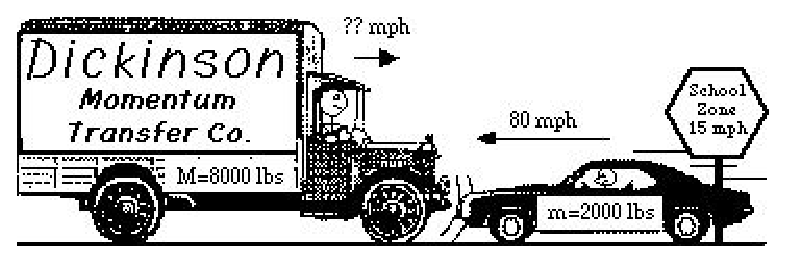
\includegraphics{momentum/momentum_fig1.eps} \par}
%\vspace{0.3cm}
{\par\centering 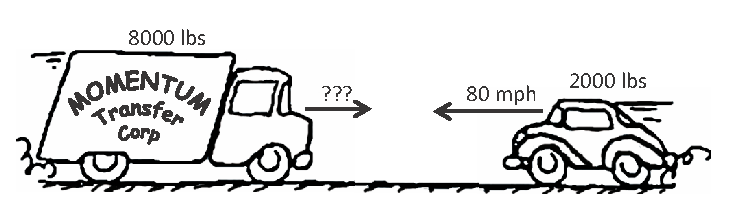
\includegraphics{momentum/car_and_van.eps} \par}

It's early fall and you are driving along a two lane highway in a rented moving
van. It is full of all of your possessions so you and the loaded truck were
weighed in at 8000 lbs. You have just slowed down to 15 MPH because you're in
a school zone. It's a good thing you thought to do that because a group of first
graders is just starting to cross the road. Just as you pass the children you
see a 2000 lb sports car in the oncoming lane heading straight for the children
at about 80 MPH. What a fool the driver is! A desperate thought crosses your
mind. You figure that you just have time to swing into the oncoming lane and
speed up a bit before making a head-on collision with the sports car. You want
your truck and the sports car to crumple into a heap that sticks together and
doesn't move. Can you save the children or is this just a suicidal act? For
simulated observations of this situation you can use two carts of different
masses set up to stick together in trial collisions. 

\textbf{Activity 1: Can You Stop the Car?} 

(a) Predict how fast you would have to be going to completely stop the sports
car. Explain the reasons for your prediction.
\vspace{20mm}

(b) Try some head on collisions with the carts of different masses to simulate
the event. Describe some of your observations. What happens when the less massive
cart is moving much faster than the more massive cart? Much slower? At about
the same speed?
\vspace{20mm}

(c) Based on your intuitive answers in parts (a) and (b) and your observations,
what mathematical definition might you use to describe the momentum (or motion)
of a moving vehicle traveling with a known mass and velocity?
\vspace{20mm}

Just to double check your reasoning, you should have come to the conclusion
that momentum is defined by the vector equation
\[
{\vec p}=m{\vec v}.\]


\textbf{Expressing Newton's Second Law Using Momentum }

Originally Newton did not use the concept of acceleration or velocity in his
laws. Instead he used the term ``motion,'' which he defined
as the product of mass and velocity (a quantity we now call momentum). Let's
examine a translation from Latin of Newton's first two laws (with some parenthetical
changes for clarity).

\textit{Newton's First Two Laws of Motion}

\begin{enumerate}
\item \textit{Every body continues in its state of rest, or of uniform motion in a
right line, unless it is compelled to change that state by forces impressed
on it. }
\item \textit{The (rate of) change of motion is proportional to the motive force impressed:
and is made in the direction in which that force is impressed.}
\end{enumerate}
The more familiar contemporary statement of the second law is that the net force
on an object is the product of its mass and its acceleration where the direction
of the force and of the resulting acceleration are the same. Newton's statement
of the law and the more modern statement are mathematically equivalent, as you
will show.

\textbf{Activity 2: Re-expressing Newton's Second Law} 

(a) Write down the contemporary mathematical expression for Newton's second
law relating net force to mass and acceleration. Please use vector signs and
a summation sign where appropriate.
\vspace{10mm}

(b) Write down the definition of instantaneous acceleration in terms of the
rate of change of velocity. Again, use vector signs.
\vspace{10mm}

(c) If an object has a changing velocity and a constant
mass then \( m\frac{d{\vec v}}{dt}=\frac{d\left( m{\vec v}\right) }{dt} \).
Explain why.
\vspace{20mm}

(d) Show that \( \sum {\vec F}=m{\vec a}=\frac{d{\vec p}}{dt} \).
\vspace{20mm}

%(e) Explain in detail why Newton's statement of the second law and the 
%mathematical expression \( \sum {\vec F}=\frac{d{\vec p}}{dt} \) are
%two representations of the same statement, i.e., are logically equivalent.
%\vspace{20mm}

\textbf{Momentum Change and Collision Forces} 

\textit{What's Your Intuition?} 

You are sleeping in your sister's room while she is away at college. Your house
is on fire and smoke is pouring into the partially open bedroom door. The room
is so messy that you cannot get to the door. The only way to close the door
is to throw either a blob of clay or a super ball at the door --- 
there's not enough time to throw both.

\textbf{Activity 3: What Packs the Biggest Wallop-A Clay Blob or a Super ball? }

Assuming that the clay blob and the super ball have the same mass, which would
you throw to close the door: the clay blob (which will stick to the door) or
the super ball (which will bounce back with almost the same velocity it had
before it collided with the door)? Give reasons for your choice, using any notions
you already have or any new concepts developed in physics such as force, momentum,
Newton's laws, etc. Remember, your life depends on it!
\vspace{30mm}

\textbf{Momentum Changes} 

It would be nice to be able to use Newton's formulation of the second law of
motion to find collision forces, but it is difficult to measure the rate of
change of momentum during a rapid collision without special instruments. However,
measuring the momenta of objects just before and just after a collision is usually
not too difficult. This led scientists in the seventeenth and eighteenth centuries
to concentrate on the overall changes in momentum that resulted from collisions.
They then tried to relate changes in momentum to the forces experienced by an
object during a collision. In the next activity you are going to explore the
mathematics of calculating momentum changes.

\newpage

\textbf{Activity 4: Predicting Momentum Changes }

Which object undergoes the most momentum change during the collision with a
door: the clay blob or the super ball? Explain your reasoning carefully.
\vspace{20mm}

Let's check your reasoning with some formal calculations of the momentum changes
for both inelastic and elastic collisions. This is a good review of the properties
of one-dimensional vectors. Recall that momentum is defined as a vector quantity
that has both magnitude and direction. Mathematically, momentum \emph{change} 
is given by the equation
\[
\Delta {\vec p}={{\vec p}_{f}}-{{\vec p}_{i}}\]


where \( {{\vec p}_{i}} \) is the initial momentum of the object just
before and \( {{\vec p}_{f}} \) is its final momentum just after a
collision.

\textbf{Activity 5: Calculating 1D Momentum Changes} 

(a) Suppose a dead ball (or clay blob) is dropped on a table and ``sticks''
in such a way that it has an initial momentum just before it hits of 
\( {{\vec p}_{i}}=-p_{iy}\, \widehat{j} \)
where \( \widehat{ j} \) is a unit vector pointing along the positive $y$ axis.
What is the final momentum of the dead ball (after it stops on the table)? 
\vspace{15mm}

(b) Calculate the change in momentum of the dead ball as a result of its collision
with the table, using the equation above for $\Delta {\vec p}$ and the \( {{\vec p}_{i}} \) and 
\( {{\vec p}_{f}} \) from part (a). Use the same type of unit vector notation to express your 
answer. Show the calculation.
\vspace{20mm}

(c) Suppose that a live ball (or a super ball) is dropped on a table and ``bounces''
on the table in an elastic collision so that its speed just before and just
after the bounce are the same. Also suppose that just before it bounces it has
an initial momentum \( {{\vec p}_{i}}=-p_{iy}\, \widehat{j} \),
where \( \widehat{j} \)
is a unit vector pointing along the positive $y$-axis. What is the final momentum
of the ball in the same vector notation? Hint: Does the final 
\( {\vec p} \)
vector point along the $+y$ or $-y$ axis? 
\vspace{15mm}

(d) Calculate the change in momentum of the ball as a result of the collision, using the equation above for \( \Delta {\vec p} \) and the \( {{\vec p}_{i}} \) and \( {{\vec p}_{f}} \) from part (c).
Use the same type of unit vector notation to express your result. Show the calculation.
\vspace{20mm}

(e) The answer is not zero. Why? How does this result compare with your 
prediction?
\newpage

(f) Now we will do the same thing with numbers. Suppose the mass of each ball is 0.2 kg and that they are dropped from 1 m above the table. Using this value for the mass of each ball and a calculated value for the velocity of each ball just before it hits the table, 
calculate the momentum just before the collision \( {{\vec p}_{i}} \)
for each of the balls. Also calculate the momentum of each ball just after the
collision \( {{\vec p}_{f}} \) and the change in momentum \( \Delta {\vec p} \)
for each ball. Show your calculations in the space below.
\answerspace{30mm}

\textbf{Applying Newton's Second Law to the Collision Process (The Egg Toss)}

Suppose somebody tosses you a raw egg and you catch it. In physics jargon, one
would say (in a very official tone of voice) that ``the egg and the
hand have undergone an inelastic collision.'' What is the relationship
between the force you have to exert on the egg to stop it, the time it takes
you to stop it, and the momentum change that the egg experiences? You ought
to have some intuition about this matter. In more ordinary language, would you
catch an egg slowly or fast?

\bigskip
\textbf{Activity 6: Momentum Changes and Average Forces on an Egg: What's Your
Intuition?} 

(a) If you catch an egg of mass $m$ that is heading toward your hand at speed
$v$, what is the magnitude of the momentum change that it undergoes?
\answerspace{10mm}

(b) Does the total momentum change differ if you catch the egg more slowly or
is it the same?
\answerspace{10mm}

(c) Suppose the time you take to bring the egg to a stop is \( \Delta  t\).
Would you rather catch the egg in such a way that \( \Delta  t\) is small or
large? Why?
\answerspace{10mm}

(d) What do you suspect might happen to the average force you exert on the egg
while catching it when \( \Delta t \) is small?
\answerspace{20mm}

\pagebreak[2]
\vspace{0.3cm}
{\par\centering 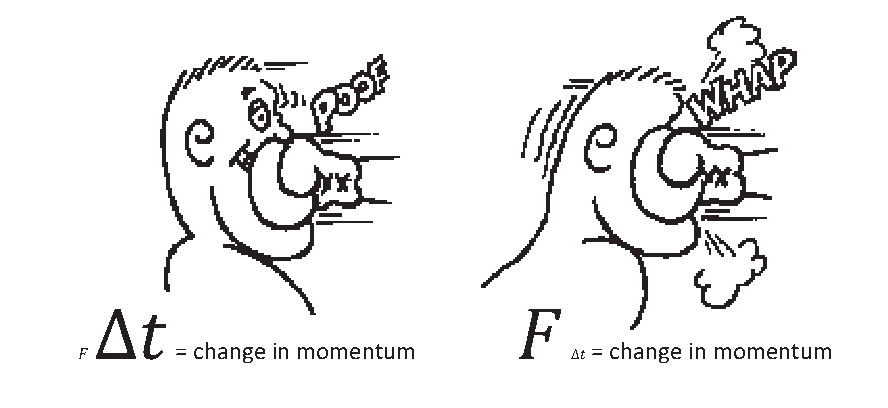
\includegraphics{momentum/momentum_fig2_new.eps} \par}
\vspace{0.3cm}

You can use Newton's second law to derive a mathematical relationship between
momentum change, force, and collision times for objects. This derivation leads
to the impulse-momentum theorem. Let's apply Newton's second law to the egg
catching scenario.

\textbf{Activity 7: Force and Momentum Change }

(a) Sketch an arrow representing the magnitude and direction of the force 
exerted by your hand on the egg as you catch it.

%\vspace{0.3cm}
%{\par\centering 
\includegraphics{momentum/momentum_fig3.eps} \par}
%\vspace{0.3cm}
{\par\centering 
\includegraphics{momentum/hand_and_egg.eps} \par}

(b) Write the mathematical expression for Newton's second law in terms of the
net force and the time rate of change of momentum. (See Activity 2(d) for 
details.)
\vspace{20mm}

%(c) Explain why, if \( {\vec F} \) is a constant 
%during the collision lasting a time \( \Delta  t\), then \( \frac{d{\vec p}}
%{dt}=\frac{\Delta {\vec p}}{\Delta t} \) for that time interval.
%\vspace{20mm}

(c) Show that for a constant force \( {\vec F} \) the change in momentum
is given by \( \Delta {\vec p}={\vec F}\,\Delta t\).  Hint: Begin with expression 
you wrote in part (b).

